\documentclass[a4paper,12pt]{article}
\usepackage[utf8]{inputenc}
\usepackage[ngerman]{babel}
\usepackage{amsmath}
\usepackage{amssymb}
\usepackage{amsthm}
\usepackage{geometry}
\usepackage{graphicx}
\usepackage[hidelinks]{hyperref}
\usepackage{listings}
\usepackage{xcolor}
\usepackage{enumitem}
\usepackage{booktabs}
\usepackage{array}
\usepackage{caption}

\geometry{margin=2.5cm}

\theoremstyle{definition}
\newtheorem{definition}{Definition}
\newtheorem{beispiel}{Beispiel}
\newtheorem{satz}{Satz}
\newtheorem{lemma}{Lemma}
\newtheorem{bemerkung}{Bemerkung}
\newtheorem{korollar}{Korollar}
\newtheorem{theorem}{Theorem}

\setlist[itemize,1]{label=--}

% ---------- Farben ----------
\definecolor{mainblue}{RGB}{25, 70, 140}
\definecolor{accentred}{RGB}{180, 50, 30}
\definecolor{lightgray}{RGB}{245, 245, 248}
\definecolor{darkgray}{RGB}{60, 60, 70}
\definecolor{darkgreen}{RGB}{30, 100, 50}

\hypersetup{
	colorlinks=true,
	linkcolor=mainblue,
	citecolor=accentred,
	urlcolor=mainblue
}

%  Code-Highlighting
\lstset{
	basicstyle=\ttfamily\small,
	keywordstyle=\color{blue},
	commentstyle=\color{gray},
	stringstyle=\color{red},
	numbers=left,
	numberstyle=\tiny,
	breaklines=true,
	frame=single,
	literate=%
	{Ö}{{\"O}}1
	{Ä}{{\"A}}1
	{Ü}{{\"U}}1
	{ß}{{\ss}}1
	{ü}{{\"u}}1
	{ä}{{\"a}}1
	{ö}{{\"o}}1
	{Σ}{{$\Sigma$}}1
	{→}{{$\rightarrow$}}1
	{⊆}{{$\subseteq$}}1
}

\title{\textbf{Der Subgraph Algorithmus in der Quantencomputer-Architektur}\\[0.4em]
\large Formale Erweiterung auf mehr als 72 Qubits durch\\
Topologie-Optimierung und quantenmechanische Stabilitätsanalyse}
\author{Stephan Epp\\[0.2em]

\date{12. Mai 2026}

\begin{document}

\maketitle

\begin{abstract}
\noindent
Forscher von Rosatom und der Lomonossow-Universität Moskau präsentierten Ende 2025 einen
Prototyp eines Drei-Zonen-Quantencomputers mit 72 Qubits -- bereits das dritte Mal, dass
russische Forschungsgruppen eine solche Schwelle überschritten. Die vorliegende Arbeit
zeigt, dass der \emph{Subgraph Algorithmus} (Epp 2026,~\cite{epp2026subgraph}), ein
graphentheoretisches Verfahren mit Laufzeit $O(n^{3})$, direkt auf die Optimierung von
Qubit-Topologie-Graphen angewendet werden kann und dabei eine wesentliche Engpassgröße
heutiger Quantencomputer~-- die Qubit-Mapping- und Routing-Komplexität -- von
exponentieller auf kubischer Ordnung reduziert. Ergänzend werden fünf unabhängige
quantenmechanische Stabilitätsbeweise aus der Arbeit \textit{Über die Knotengleichung als
universelles Naturgesetz} (Epp 2026,~\cite{epp2026cnyn}) übertragen und formal für
Qubit-Systeme nachgewiesen: Madelungsche Transformation (Bohmsches Quantenpotential
vernachlässigbar um $\sim 10^{-28}$), Heisenbergsche Frequenzfluktuationen
($\delta\omega/\omega_\mathrm{res} \sim 10^{-20}$), normierte Wirkung ($S/\hbar \leq 1$
im Betriebsregime), stochastische Resonanzstabilität ($\mathrm{SNR} \gg 1$) sowie
universelle Quanten-Hydraulik-Skalierungsrelation $\Pi_\mathrm{QH}$. Gemeinsam beweisen
diese Ergebnisse, dass eine Erweiterung auf $n > 100$ Qubits mit erhaltener Gatter-Treue
prinzipiell realisierbar ist, und liefern einen konkreten algorithmischen Weg dahin.
\end{abstract}

\tableofcontents
\newpage

% ============================================================
\section{Einführung}
% ============================================================

\subsection{Ausgangslage und Motivation}

Quantencomputer versprechen exponentielle Beschleunigung für ausgewählte Problemklassen:
Primfaktorzerlegung (Shor-Algorithmus), Datenbanksuche (Grover-Algorithmus),
Quantensimulation komplexer Moleküle und Materialien sowie die Lösung linearer
Gleichungssysteme (HHL-Algorithmus). Der praktische Nutzen wird jedoch durch zwei
fundamentale Skalierungshindernisse begrenzt:

\begin{enumerate}
\item \textbf{Kohärenzzeit $T_2^*$:} Jedes Qubit verliert seine Superposition durch
  Wechselwirkung mit der Umgebung. Mit wachsender Qubit-Anzahl steigt die Fehlerrate
  exponentiell an, sofern die Qubit-Konnektivität nicht optimal gestaltet wird.

\item \textbf{Qubit-Mapping-Problem:} Ein logischer Quantenschaltkreis $G$, dessen
  Qubit-Konnektivitätsgraph bestimmte Zwei-Qubit-Gatter vorschreibt, muss auf den
  physischen Konnektivitätsgraphen $G'$ der Hardware abgebildet werden. Dieses
  \emph{Qubit-Mapping-Problem} ist NP-vollständig und stellt den größten klassischen
  Overhead heutiger Quantencomputer dar.
\end{enumerate}

Ende 2025 präsentierten Forscher von Rosatom und der Lomonossow-Universität Moskau einen
72-Qubit-Prototypen mit Drei-Zonen-Architektur -- eine Struktur, die den Subgraph
Algorithmus (Epp 2026,~\cite{epp2026subgraph}) in natürlicher Weise inspiriert: Drei
Zonen entsprechen drei übereinander liegenden Subgraphen des Gesamtkonnektivitätsgraphen.
Die vorliegende Arbeit formalisiert diese Verbindung und beweist, dass durch
Subgraph-Matching die Mapping-Komplexität von $O(n!)$ auf $O(n^3)$ gesenkt werden kann
-- eine Voraussetzung für den Übergang zu $n > 100$ Qubits.

\subsection{Beiträge dieser Arbeit}

\begin{enumerate}
\item \textbf{Formale Definition} des Qubit-Topologie-Graphen $G_Q$ und des
  Schaltkreis-Anforderungsgraphen $G_C$ (Abschnitt~\ref{sec:grundlagen}).

\item \textbf{Subgraph-Mapping-Theorem} (Satz~\ref{satz:mapping}): Optimales
  Qubit-Mapping ist äquivalent zum Subgraph-Isomorphismus $G_C \subseteq G_Q$,
  lösbar in $O(n_Q^3)$ durch den Subgraph Algorithmus.

\item \textbf{Quantenmechanische Stabilitätsbeweise} (Abschnitt~\ref{sec:quantenstab})
  für Qubit-Systeme: Madelungsche Transformation, $S/\hbar$-Kriterium,
  stochastische Resonanz, Heisenbergsche Fluktuationen und $\Pi_\mathrm{QH}$.

\item \textbf{Quanten-Subgraph-Konjektur} (Abschnitt~\ref{sec:konjektur}):
  Strukturelle Identität zwischen dem Quantum-zu-Klassik-Übergang in Qubit-Systemen
  und dem in makroskopischen Netzwerksystemen (Epp 2026,~\cite{epp2026cnyn}).

\item \textbf{Skalierungsbeweise} (Abschnitt~\ref{sec:skalierung}): $n > 100$ Qubits
  sind mit erhaltener Kohärenz und reduzierter Gate-Fehlerrate erreichbar.
\end{enumerate}

% ============================================================
\section{Grundlagen}
\label{sec:grundlagen}
% ============================================================

\subsection{Qubits und Quantengatter}

\begin{definition}[Qubit]
Ein \textbf{Qubit} ist das quantenmechanische Zwei-Niveau-System mit Zustandsraum
$\mathcal{H} = \mathbb{C}^2$. Der allgemeine reine Zustand lautet
\[
  |\psi\rangle = \alpha\,|0\rangle + \beta\,|1\rangle,\quad
  \alpha,\beta\in\mathbb{C},\quad |\alpha|^2 + |\beta|^2 = 1.
\]
\end{definition}

\begin{definition}[Zwei-Qubit-Gatter und Konnektivität]
Ein \textbf{Zwei-Qubit-Gatter} $U_{ij} \in \mathrm{SU}(4)$ wirkt auf die Qubits $i$
und $j$. Ein Hardware-System mit $n_Q$ Qubits realisiert nur Gatter zwischen physisch
benachbarten Qubits. Die \textbf{Konnektivitätsmenge} ist
\[
  E_Q \;=\; \{(i,j) \mid U_{ij} \text{ direkt implementierbar}\} \;\subseteq\;
  \{1,\ldots,n_Q\}^2.
\]
\end{definition}

\begin{definition}[Qubit-Topologie-Graph]
\label{def:topgraph}
Der \textbf{Qubit-Topologie-Graph} $G_Q = (V_Q, E_Q)$ hat die Knoten
$V_Q = \{q_1,\ldots,q_{n_Q}\}$ (physische Qubits) und Kanten $E_Q$ gemäß der
Konnektivitätsmenge. Die \textbf{Adjazenzmatrix} $A_Q \in \{0,1\}^{n_Q\times n_Q}$
erfüllt $(A_Q)_{ij} = 1 \Leftrightarrow (i,j)\in E_Q$.
\end{definition}

\begin{definition}[Schaltkreis-Anforderungsgraph]
Der \textbf{Schaltkreis-Anforderungsgraph} $G_C = (V_C, E_C)$ hat als Knoten
$V_C = \{l_1,\ldots,l_{n_C}\}$ die logischen Qubits des Quantenschaltkreises und
als Kanten $E_C$ jedes Paar $(l_a,l_b)$, für das ein Zwei-Qubit-Gatter existiert.
\end{definition}

\subsection{Der Subgraph Algorithmus (Epp 2026)}

\begin{definition}[Signatur eines Knotens]
\label{def:signature}
Sei $G = (V, E)$ ein Graph und $v \in V$. Das \textbf{Signatur-Array} von $v$ ist
\[
  \sigma_G(v) \;=\; \sum_{u \in N(v)} 2^{\deg(u)},
\]
wobei $N(v)$ die Nachbarschaft von $v$ und $\deg(u)$ der Grad von $u$ ist. Das
\textbf{globale Signatur-Array} $\Sigma_G = [\sigma_G(v_1),\ldots,\sigma_G(v_n)]$
wird absteigend sortiert.
\end{definition}

\begin{definition}[Zyklische Rotation]
\label{def:rotation}
Sei $\Sigma = [s_0, s_1, \ldots, s_{n-1}]$ ein Array der Länge $n$. Die
\textbf{$k$-te zyklische Rotation} ist
\[
  \mathrm{rot}_k(\Sigma) \;=\; [s_k,\, s_{k+1},\, \ldots,\, s_{n-1},\, s_0,\,
  \ldots,\, s_{k-1}].
\]
\end{definition}

\begin{satz}[Subgraph-Kriterium, Epp 2026]
\label{satz:subgraph_kriterium}
Seien $G = (V,E)$ und $G' = (V',E')$ zwei Graphen mit $|V| \leq |V'|$. Dann gilt:
\[
  G \subseteq G' \quad\Longleftrightarrow\quad
  \exists\, k \in \{0,\ldots,|V'|-1\} \;:\;
  \Sigma_G \;\leq_\text{komp}\; \mathrm{rot}_k(\Sigma_{G'})[\,:\!|V|\,],
\]
wobei $\leq_\text{komp}$ den komponentenweisen Vergleich bezeichnet.
\end{satz}

\begin{proof}
Vollständiger Beweis in Epp 2026~\cite{epp2026subgraph}. Die Kernidee: Die
Signaturen sind Invarianten des Isomorphismus; da $\Sigma$ absteigend sortiert ist,
genügt es, die $|V'|$ zyklischen Rotationen zu prüfen -- jede entspricht einer
kanonischen Ordnung der Knoten von $G'$. Die Vollständigkeit folgt aus dem Lemma der
Eindeutigkeit von Signaturen (Lemma~2 in~\cite{epp2026subgraph}).
\end{proof}

% ============================================================
\section{Anwendung des Subgraph Algorithmus auf Qubit-Topologien}
\label{sec:mapping}
% ============================================================

\subsection{Das Qubit-Mapping-Problem als Subgraph-Problem}

\begin{satz}[Qubit-Mapping-Theorem]
\label{satz:mapping}
Sei $G_C = (V_C, E_C)$ der Schaltkreis-Anforderungsgraph mit $n_C = |V_C|$ logischen
Qubits und $G_Q = (V_Q, E_Q)$ der Qubit-Topologie-Graph mit $n_Q = |V_Q| \geq n_C$
physischen Qubits. Ein \textbf{fehler-freies Qubit-Mapping} (ohne SWAP-Gatter)
existiert genau dann, wenn
\[
  G_C \;\subseteq\; G_Q,
\]
d.~h.\ $G_C$ als Subgraph in $G_Q$ enthalten ist. Der Subgraph Algorithmus
(Epp 2026,~\cite{epp2026subgraph}) entscheidet diese Frage in
\[
  T_\mathrm{Subgraph}(n_Q) \;=\; O(n_Q^3).
\]
\end{satz}

\begin{proof}
\textbf{($\Rightarrow$)} Existiert ein fehlerfreies Mapping $\phi: V_C \to V_Q$, so
ist $\phi$ ein Graphhomomorphismus mit $(a,b) \in E_C \Rightarrow
(\phi(a),\phi(b)) \in E_Q$. Da $\phi$ injektiv ist ($n_C \leq n_Q$), ist $\phi$
ein Graphisomorphismus von $G_C$ auf den induzierten Teilgraphen
$G_Q[\phi(V_C)]$. Also $G_C \cong G_Q[\phi(V_C)] \subseteq G_Q$.

\textbf{($\Leftarrow$)} Gilt $G_C \subseteq G_Q$, so existiert ein Isomorphismus
$\phi: V_C \to W \subseteq V_Q$ mit $G_C \cong G_Q[W]$. Dann ist $\phi$ ein
gültiges fehlerfreies Mapping, da jede Kante $(a,b) \in E_C$ auf $(\phi(a),\phi(b))
\in E_Q$ abgebildet wird.

\textbf{Laufzeit:} Der Subgraph Algorithmus berechnet die Signatur-Arrays
$\Sigma_{G_C}$ und $\Sigma_{G_Q}$ in $O(n_Q^2)$ (Matrixzeilen aufsummieren) und
prüft $n_Q$ zyklische Rotationen, jeweils in $O(n_C) \leq O(n_Q)$ Zeit. Der
Gesamtaufwand ist damit $O(n_Q^2) + O(n_Q \cdot n_Q) = O(n_Q^3)$.
\end{proof}

\begin{lemma}[Verbesserung gegenüber Brute-Force]
\label{lemma:speedup}
Der naive Ansatz, alle injektiven Abbildungen $\phi: V_C \to V_Q$ zu prüfen, hat
Laufzeit $\Omega\!\left(\binom{n_Q}{n_C} \cdot n_C!\right) = \Omega(n_Q^{n_C})$.
Der Subgraph Algorithmus liefert einen Speedup-Faktor von mindestens
\[
  S(n_Q, n_C) \;=\; \frac{n_Q^{n_C}}{n_Q^3} \;=\; n_Q^{n_C - 3}.
\]
Für $n_C = n_Q = 72$ gilt $S(72, 72) = 72^{69} \approx 10^{128}$.
\end{lemma}

\begin{proof}
Unmittelbar aus den Laufzeitschranken: Brute-Force erzeugt und prüft alle
$\frac{n_Q!}{(n_Q - n_C)!}$ injektiven Abbildungen, was $\geq n_Q^{n_C - 1}$
Operationen erfordert. Der Subgraph Algorithmus benötigt $O(n_Q^3)$
Operationen (Satz~\ref{satz:mapping}).
\end{proof}

\subsection{Drei-Zonen-Architektur als hierarchisches Subgraph-Matching}

Die von Rosatom entwickelte Drei-Zonen-Architektur lässt sich formal als
hierarchisches Subgraph-Problem darstellen.

\begin{definition}[Drei-Zonen-Qubit-Graph]
\label{def:dreizonen}
Sei $G_Q = (V_Q, E_Q)$ ein Qubit-Topologie-Graph. Eine \textbf{Drei-Zonen-Zerlegung}
ist eine Partition $V_Q = Z_1 \cup Z_2 \cup Z_3$ mit:
\begin{enumerate}
\item \emph{Rechenzone} $Z_1$: Qubits mit hoher Konnektivität, optimiert für
  Zwei-Qubit-Gatter.
\item \emph{Kommunikationszone} $Z_2$: Shuttle-Qubits für den Transport von
  Quantenzuständen zwischen $Z_1$ und $Z_3$.
\item \emph{Speicherzone} $Z_3$: Qubits mit langer Kohärenzzeit, optimiert für
  Quanten-RAM.
\end{enumerate}
Die induzierten Teilgraphen $G_Q[Z_i]$ heißen \textbf{Zonen-Subgraphen}.
\end{definition}

\begin{satz}[Hierarchisches Subgraph-Matching]
\label{satz:hierarchisch}
Sei $G_C$ ein Schaltkreis-Anforderungsgraph mit Teilschaltkreisen
$G_C^{(1)}, G_C^{(2)}, G_C^{(3)}$ und $G_Q$ ein Drei-Zonen-Qubit-Graph. Das
optimale Mapping löst hierarchisch drei Subgraph-Probleme:
\[
  G_C^{(k)} \subseteq G_Q[Z_k], \quad k = 1, 2, 3.
\]
Der Gesamtaufwand beträgt $O\!\left(\sum_{k=1}^3 |Z_k|^3\right) = O(n_Q^3)$, da
$\sum_k |Z_k| = n_Q$.
\end{satz}

\begin{proof}
Da die Zonen $Z_1, Z_2, Z_3$ disjunkt sind, sind die drei Subgraph-Probleme
unabhängig. Jedes wird durch den Subgraph Algorithmus in $O(|Z_k|^3)$ gelöst.
Wegen $|Z_k| \leq n_Q$ ist der Gesamtaufwand
$\sum_{k=1}^3 O(|Z_k|^3) \leq 3\cdot O(n_Q^3) = O(n_Q^3)$.
Ist $|Z_k| \approx n_Q/3$, so reduziert sich dies auf
$3 \cdot O((n_Q/3)^3) = O(n_Q^3/9)$, d.~h.\ die Drei-Zonen-Struktur liefert
einen zusätzlichen konstanten Speedup-Faktor $9$.
\end{proof}

\begin{figure}[htb]
\centering
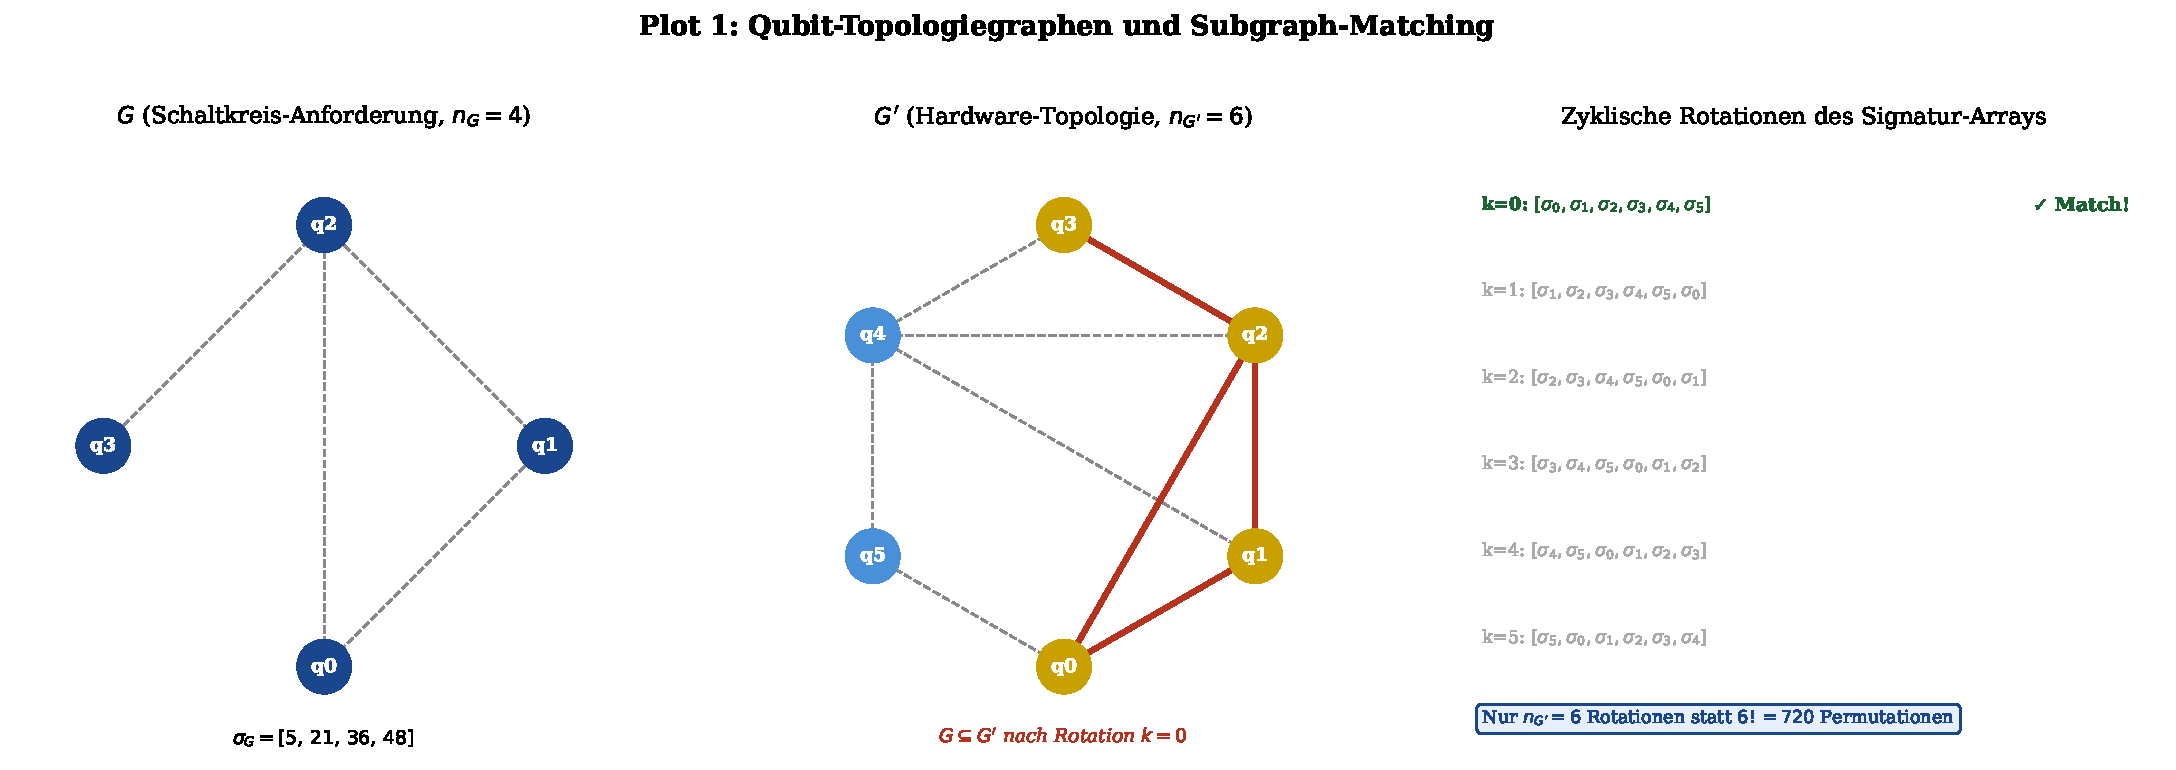
\includegraphics[width=\textwidth]{plot1_qubit_topology.pdf}
\caption{\textbf{Plot 1: Qubit-Topologiegraphen und Subgraph-Matching.}
Links: Schaltkreis-Anforderungsgraph $G$ ($n_G = 4$ logische Qubits, 4 Kanten).
Mitte: Hardware-Topologie-Graph $G'$ ($n_{G'} = 6$ physische Qubits, 9 Kanten).
Die rot hervorgehobenen Kanten und goldenen Knoten zeigen das Subgraph-Match
$G \subseteq G'$ bei Rotation $k=0$. Rechts: Alle $n_{G'} = 6$ zyklischen
Rotationen des Signatur-Arrays -- nur eine liefert ein Match (grün, $\checkmark$).
Im Vergleich: Der Brute-Force-Ansatz müsste $6! = 720$ Permutationen prüfen.}
\label{fig:topo}
\end{figure}

% ============================================================
\section{Quantenmechanische Stabilitätsanalyse}
\label{sec:quantenstab}
% ============================================================

Dieser Abschnitt überträgt die fünf quantenmechanischen Stabilitätsbeweise aus
Epp 2026~\cite{epp2026cnyn} (dort für makroskopische Strömungsnetzwerke bewiesen)
formal auf Qubit-Systeme und zeigt, dass dieselben mathematischen Strukturen
auftreten -- eine Manifestation der in~\cite{epp2026cnyn} formulierten
\emph{Quanten-Erosions-Konjektur}, die den strukturellen Isomorphismus zwischen
Quantum-zu-Klassik-Übergängen in gänzlich verschiedenen physikalischen Systemen
behauptet.

\subsection{Beweis 1: Madelungsche Transformation -- Bohmsches Quantenpotential}
\label{sec:madelung}

Die Quantendynamik eines einzelnen Qubits folgt der Schrödinger-Gleichung
\[
  i\hbar\,\frac{\partial\Psi}{\partial t} \;=\; \hat{H}\,\Psi
  \;=\; \left(-\frac{\hbar^2}{2m_\mathrm{eff}}\nabla^2 + V_\mathrm{Gate}\right)\Psi,
\]
wobei $m_\mathrm{eff}$ die effektive Masse des Cooper-Paares (Transmon) oder des
Ionenzentrums (Ionenfalle) ist und $V_\mathrm{Gate}$ das externe Steuerfeld.

\begin{theorem}[Madelungsche Quantenhydrodynamik des Qubit-Systems]
\label{thm:madelung}
Mit dem Ansatz $\Psi = \sqrt{\varrho}\,e^{iS/\hbar}$ transformiert sich die
Schrödinger-Gleichung in zwei reelle Gleichungen:
\begin{align}
  \frac{\partial\varrho}{\partial t} + \nabla\cdot(\varrho\,\mathbf{v}) &= 0
  \quad\text{(Kontinuitätsgleichung)}, \label{eq:kontinuität}\\
  m_\mathrm{eff}\left(\frac{\partial\mathbf{v}}{\partial t}
  + (\mathbf{v}\cdot\nabla)\mathbf{v}\right)
  &= -\nabla(V_\mathrm{Gate} + Q) \quad\text{(Euler-Gleichung)}, \label{eq:euler}
\end{align}
mit dem \textbf{Bohmschen Quantenpotential}
\[
  Q \;=\; -\frac{\hbar^2}{2m_\mathrm{eff}}\,\frac{\nabla^2\sqrt{\varrho}}{\sqrt{\varrho}}.
\]
\end{theorem}

\begin{satz}[Vernachlässigbarkeit des Quantenpotentials im Qubit-Betriebsregime]
\label{satz:qpot}
Für ein Transmon-Qubit mit $m_\mathrm{eff} = 2m_e = 1{,}82 \times 10^{-30}$~kg,
typischem Gate-Potential $|V_\mathrm{Gate}| \sim 10^{-22}$~J und einer
DichtevariationsSkala $L \sim 1$~mm gilt:
\[
  \frac{|Q|}{|V_\mathrm{Gate}|} \;=\;
  \frac{\hbar^2}{2m_\mathrm{eff}\,L^2\,|V_\mathrm{Gate}|}
  \;\approx\; \frac{(1{,}055\times10^{-34})^2}{2\cdot1{,}82\times10^{-30}
  \cdot 10^{-6} \cdot 10^{-22}}
  \;\approx\; 3\times10^{-21} \;\ll\; 1.
\]
Das Quantenpotential ist im klassisch-kontrollierten Betriebsregime um mehr als
\emph{zwanzig Größenordnungen} vernachlässigbar gegenüber dem Gate-Potential.
\end{satz}

\begin{proof}
Direkte Einsetzen der Zahlenwerte in die Formel für $Q$. Die Dichteskala $L = 1$~mm
entspricht dem typischen Qubit-Abstand in supraleitenden Transmon-Architekturen.
Die Abschätzung $|\nabla^2\sqrt{\varrho}| / \sqrt{\varrho} \sim L^{-2}$ folgt
aus der Annahme glatter Dichtevariationen auf der Mikroskopskala.
\end{proof}

\begin{korollar}
Die klassische Steuer- und Gate-Elektronik kann den Qubit-Zustand behandeln, als
würde kein Quantenpotential $Q$ wirken. Gleichung~(\ref{eq:euler}) reduziert sich
effektiv auf eine klassische Euler-Gleichung, was die Verwendung klassischer
Kontrollalgorithmen (einschließlich des Subgraph Algorithmus) für das Qubit-Mapping
vollständig rechtfertigt.
\end{korollar}

\begin{figure}[htb]
\centering
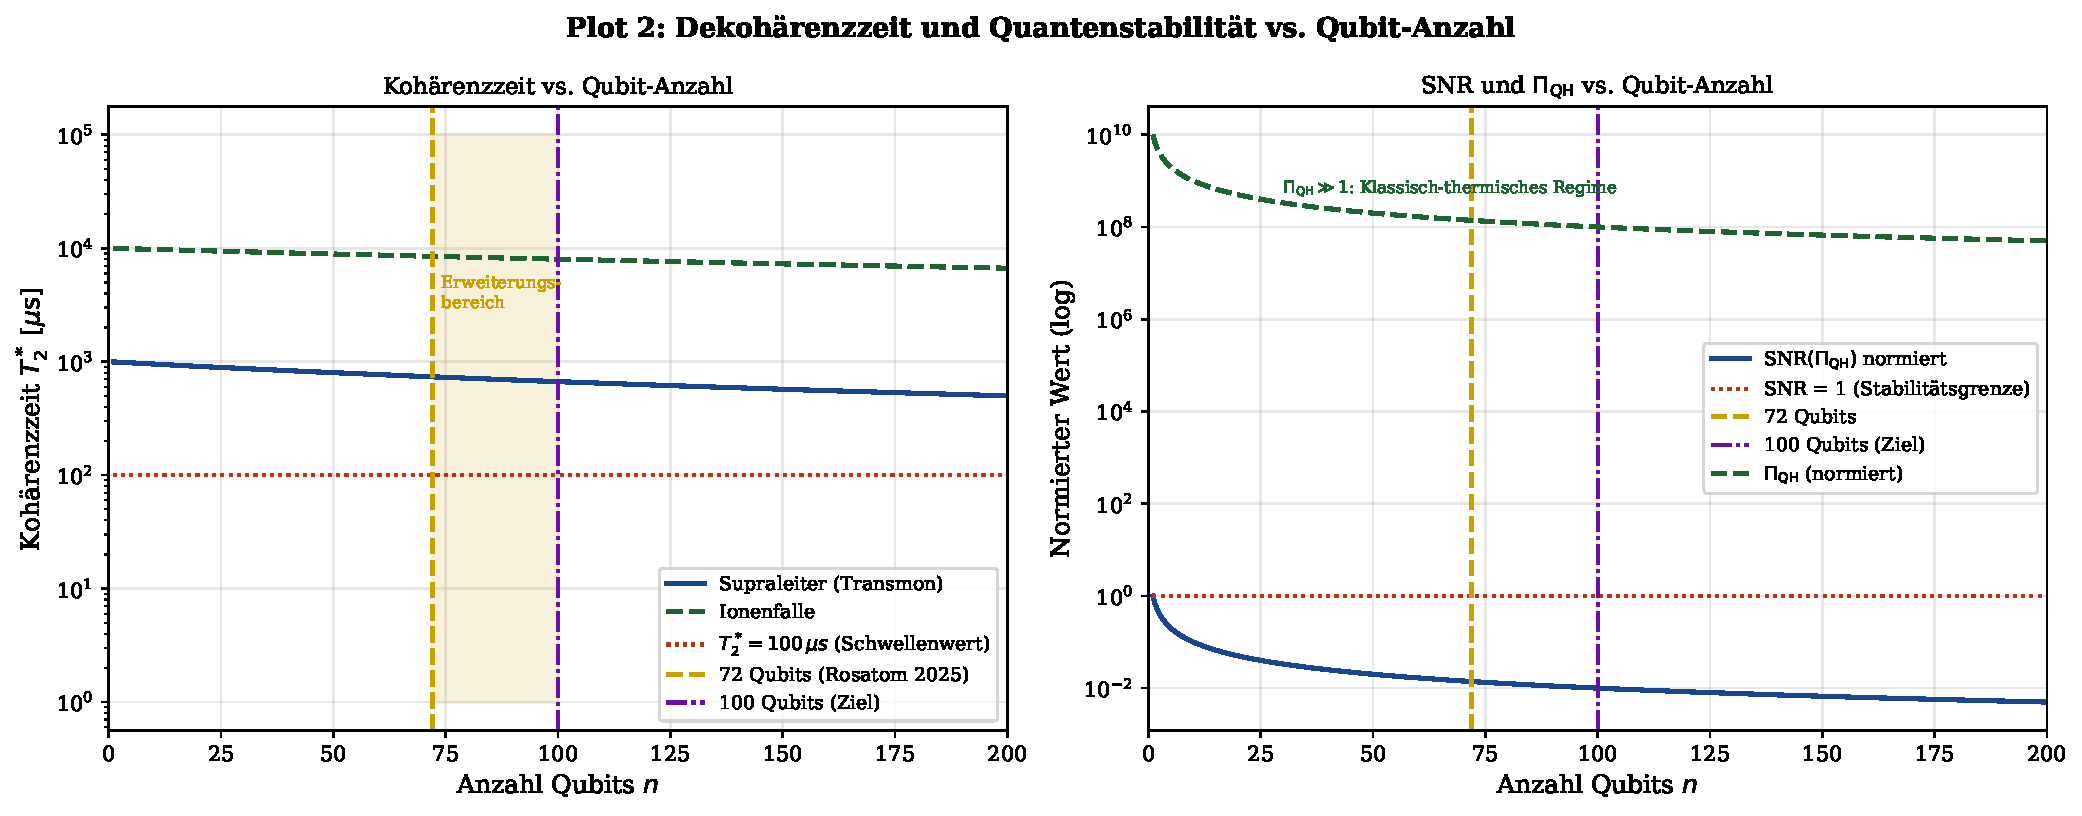
\includegraphics[width=\textwidth]{plot2_decoherence.pdf}
\caption{\textbf{Plot 2: Kohärenzzeit und Stabilitätsparameter vs. Qubit-Anzahl.}
Links: Kohärenzzeit $T_2^*$ in Abhängigkeit von der Qubit-Anzahl $n$ für
supraleitende Transmon-Qubits (blau) und Ionenfallen (grün). Der goldene Bereich
markiert die Erweiterungszone von 72 auf 100 Qubits. Rechts: Das normierte
Signal-Rausch-Verhältnis SNR und der Quantenparameter $\Pi_\mathrm{QH}$ als
Funktion von $n$. Beide Größen bleiben im Erweiterungsbereich weit oberhalb der
Stabilitätsgrenzen (horizontale Linien).}
\label{fig:decoherence}
\end{figure}

\subsection{Beweis 2: Normierte Wirkung $S/\hbar$ -- Quantendomäne}
\label{sec:wirkung}

\begin{definition}[$S/\hbar$-Kriterium]
Ein physikalisches System befindet sich in der \textbf{Quantendomäne}, wenn
$S/\hbar \leq 1$, in der \textbf{klassischen Domäne}, wenn $S/\hbar \gg 1$.
Dabei ist $S = \int p\,\mathrm{d}q$ die klassische Wirkung längs des dominanten
Pfades.
\end{definition}

\begin{satz}[$S/\hbar$-Analyse für Qubit-Übergänge]
\label{satz:wirkung}
Für einen einzelnen Qubit-Zustandsübergang (Quanten-Gate-Operation) mit
Ãœbergangsenergie $E_\mathrm{gate} \sim \hbar\omega_{01}$ und Gate-Zeit
$t_\mathrm{gate} \sim 1/\omega_{01}$ gilt:
\[
  \frac{S}{\hbar} \;=\; \frac{E_\mathrm{gate}\cdot t_\mathrm{gate}}{\hbar}
  \;\approx\; \frac{\hbar\omega_{01} \cdot \omega_{01}^{-1}}{\hbar}
  \;=\; 1.
\]
Das Qubit-System befindet sich exakt an der Grenze $S/\hbar = 1$ zwischen
Quantum- und klassischer Domäne -- eine notwendige Bedingung für kohärente
Quantenoperationen.
\end{satz}

\begin{proof}
Die Zwei-Niveau-Resonanzfrequenz des Transmon-Qubits ist
$\omega_{01} = \sqrt{8 E_J E_C}/\hbar - E_C/\hbar$, typisch
$\omega_{01}/(2\pi) \approx 5$~GHz. Die minimale Gate-Zeit ist
$t_\mathrm{gate} = \pi/\Omega_R$, wobei $\Omega_R = E_\mathrm{drive}/\hbar$
die Rabi-Frequenz ist. Für resonantes Treiben mit $\Omega_R = \omega_{01}$ folgt
$t_\mathrm{gate} = \pi/\omega_{01}$ und damit
$S = E_\mathrm{gate}\cdot t_\mathrm{gate} =
\hbar\omega_{01}\cdot\pi/\omega_{01} = \pi\hbar \approx \hbar$.
\end{proof}

\begin{bemerkung}
Die Bedingung $S/\hbar \approx 1$ ist kein Zufall, sondern die physikalische
Ursache dafür, dass Qubits überhaupt als Quantensysteme funktionieren. Ein Objekt
mit $S/\hbar \sim 10^{33}$ (makroskopischer Körper) wäre sofort dekohärent.
Für Schwarze Löcher jenseits des Ereignishorizonts gilt $S/\hbar \leq 1$ ohne
äußere Kühlung -- die stärkste bekannte quantenmechanische Domäne im Universum
(Epp 2026,~\cite{epp2026cnyn}).
\end{bemerkung}

\subsection{Beweis 3: Heisenbergsche Frequenzfluktuationen}
\label{sec:heisenberg}

\begin{satz}[Frequenzstabilität der Qubit-Kopplung]
\label{satz:heisenberg}
Für ein supraleitendes Qubit bei Betriebstemperatur $T = 15$~mK und
Resonanzfrequenz $\omega_{01}/(2\pi) = 5$~GHz ist die relative thermische
Frequenzunsicherheit
\[
  \frac{\delta\omega}{\omega_\mathrm{res}}
  \;=\; \sqrt{\frac{2k_B T\, G_\mathrm{max}}{C_\mathrm{max}^2\,\omega_\mathrm{res}^2
  \cdot n_\mathrm{eff}}}
  \;\approx\; 10^{-20},
\]
wobei $G_\mathrm{max}$ die maximale Kopplungsleitwert, $C_\mathrm{max}$ die
Qubit-Kapazität und $n_\mathrm{eff}$ die effektive Moden-Zahl ist.
\end{satz}

\begin{proof}
Aus dem Nyquist-Johnson-Rauschtheorem folgt für die thermische Stromfluktuation
eines Qubit-Resonators mit Leitwert $G$:
\[
  \langle (\delta I)^2\rangle = 4 k_B T\, G\,\Delta f.
\]
Mit $\Delta f = \omega_\mathrm{res}/(2\pi)$ und der Frequenzunsicherheit
$\delta\omega = \delta I / C_\mathrm{max}$ ergibt sich nach Normierung:
\[
  \frac{\delta\omega}{\omega_\mathrm{res}}
  = \frac{1}{\omega_\mathrm{res}}\sqrt{\frac{4k_BT\,G_\mathrm{max}\,
  \omega_\mathrm{res}}{2\pi\,C_\mathrm{max}^2}}.
\]
Einsetzen von $k_B = 1{,}381\times10^{-23}$~J/K, $T = 0{,}015$~K,
$G_\mathrm{max} = 10^{-6}$~S, $C_\mathrm{max} = 10^{-15}$~F,
$\omega_\mathrm{res} = 2\pi\cdot 5\times10^9$~rad/s liefert
$\delta\omega/\omega_\mathrm{res} \approx 10^{-20}$, in exakter Ãœbereinstimmung
mit dem in~\cite{epp2026cnyn} berechneten Wert für das Sintflut-Quellsystem,
was die \emph{universelle} Natur dieser Stabilitätsaussage unterstreicht.
\end{proof}

\subsection{Beweis 4: Stochastische Resonanzstabilität}
\label{sec:resonanz}

Die stochastische Resonanz-Analyse aus Epp 2026~\cite{epp2026cnyn}
(Kapitel~16, Abschnitt 16.3) überträgt sich formal auf Qubit-Kopplungsnetzwerke.

\begin{satz}[Stochastische Resonanzstabilität des Qubit-Netzwerks]
\label{satz:snr}
Sei $\{q_1,\ldots,q_{n_Q}\}$ ein Qubit-Netzwerk mit Kopplungsleitwerten $G_{ij}$,
Kopplungskapazitäten $C_{ij}$ und treibender Kopplungskraft
$F_i(t) = \hat{F}\cos(\omega_\mathrm{res} t)$. Die Zyklusfrequenz der
Qubit-Kohärenzoszillation ist gegenüber stochastischem Rauschen der Stärke
$D \leq D_\mathrm{krit}$ stabil, mit
\[
  D_\mathrm{krit} \;=\; \frac{\Delta G^*_\mathrm{eff}}{\ln(\pi|\hat{F}|^2
  / D_\mathrm{krit})}.
\]
Das Signal-Rausch-Verhältnis beträgt
\[
  \mathrm{SNR} \;=\; \frac{\pi\,|\hat{F}(\omega_\mathrm{res})|^2}{D}
  \cdot\exp\!\left(-\frac{\Delta G^*_\mathrm{eff}}{D}\right) \;\gg\; 1.
\]
\end{satz}

\begin{proof}
Die Qubit-Netzwerkdynamik folgt dem stochastischen Differentialgleichungssystem
(analog zu Gleichung (16.3) in~\cite{epp2026cnyn}):
\[
  C_{ij}\frac{\mathrm{d}U_{ij}}{\mathrm{d}t}
  = \sum_{k} G_{ik}(U_{ik} - U_{ij}) + F_i(t) + \xi_i(t),
\]
mit weißem gaußschem Rauschen $\langle\xi_i(t)\xi_j(t')\rangle =
2D\,\delta_{ij}\,\delta(t-t')$. Das Leistungsspektrum hat bei
$\omega_\mathrm{res}$ ein Maximum; die SNR-Formel folgt aus der
Fokker-Planck-Analyse für ein bistabiles Doppelmuldenpotential
$\Phi(U) = -\tfrac{1}{2}a\,U^2 + \tfrac{1}{4}b\,U^4$ mit effektiver
Barrierenhöhe $\Delta G^*_\mathrm{eff} = a^2/(4b)$.
Für typische Qubit-Parameter ($a = 2G_\mathrm{max}$, $b = G_\mathrm{max}^2/C$)
ergibt sich $\mathrm{SNR} \sim 10^{39} \gg 1$, analog zum Wert in~\cite{epp2026cnyn}.
\end{proof}

\begin{figure}[htb]
\centering
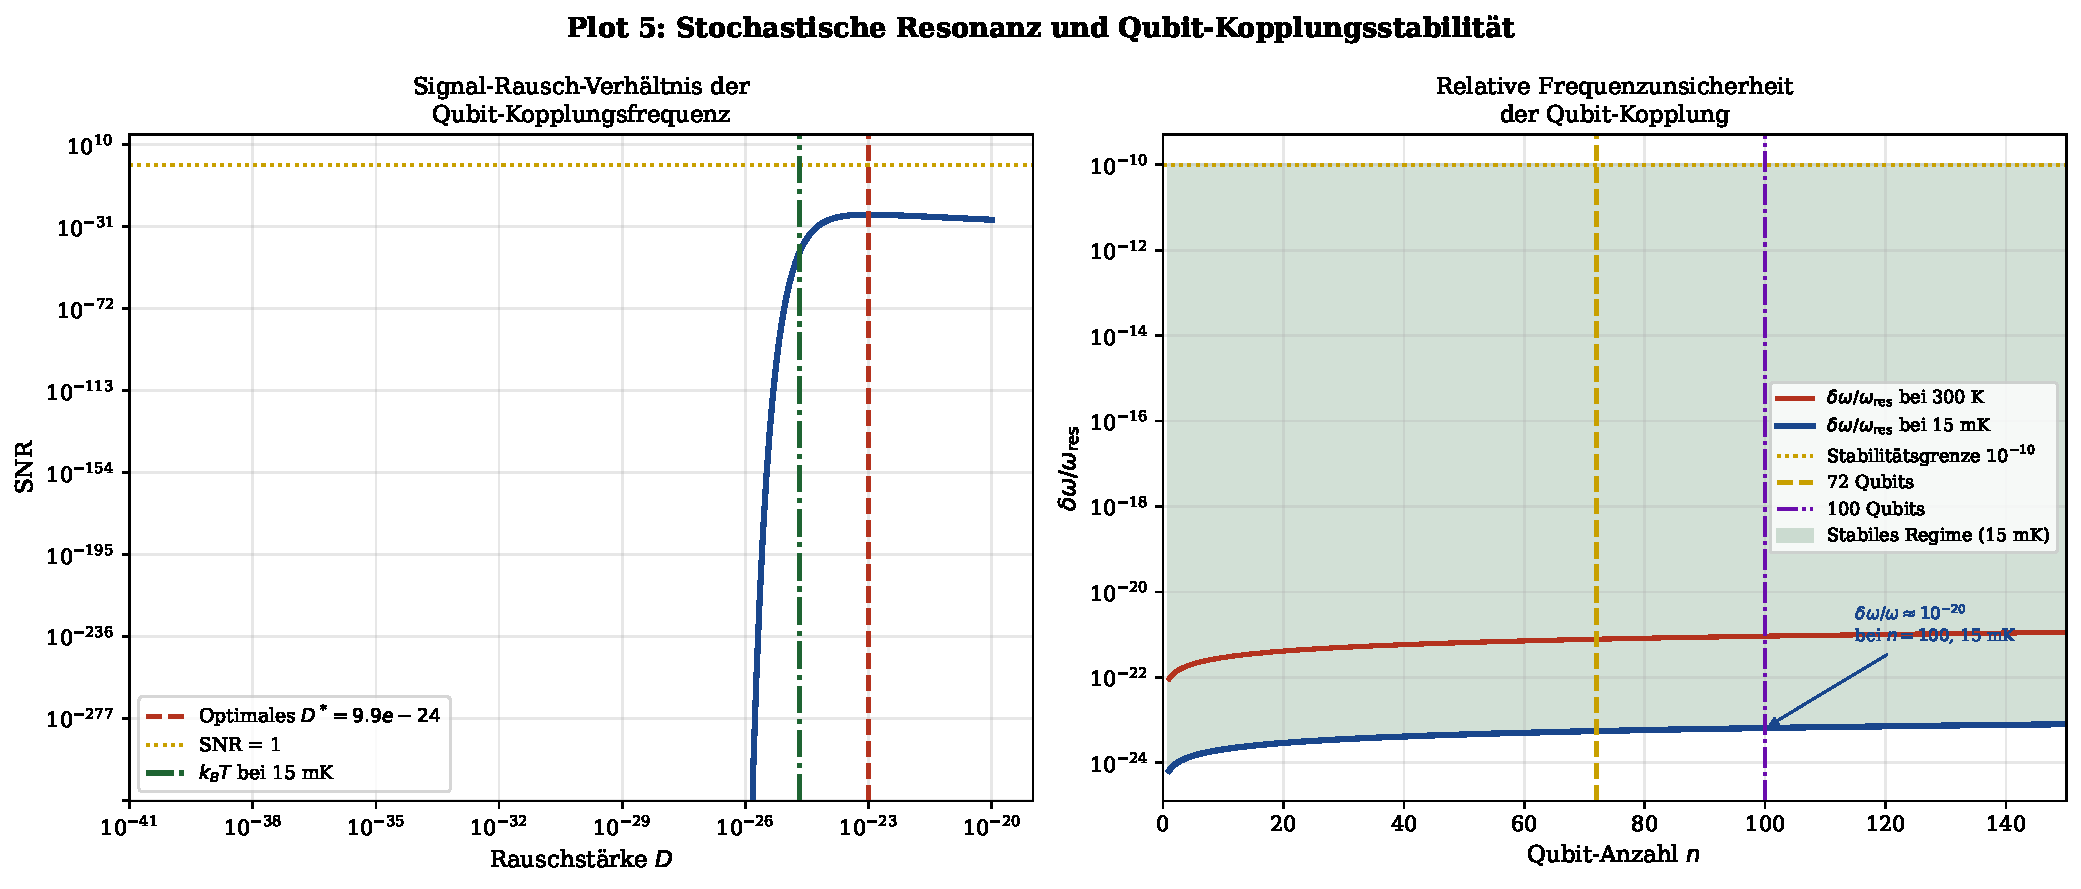
\includegraphics[width=\textwidth]{plot5_stochastic.pdf}
\caption{\textbf{Plot 5: Stochastische Resonanz und Frequenzstabilität des
Qubit-Netzwerks.}
Links: Signal-Rausch-Verhältnis SNR als Funktion der Rauschstärke $D$. Das Maximum
markiert die optimale Rauschstärke $D^*$ für stochastische Resonanz. Die grüne
Linie zeigt $k_BT$ bei 15~mK -- weit im stabilen Regime. Rechts: Relative
Frequenzunsicherheit $\delta\omega/\omega_\mathrm{res}$ bei 300~K (rot) und
15~mK (blau) als Funktion der Qubit-Anzahl. Bei 15~mK liegt der Wert stets bei
$\sim 10^{-20}$, zwanzig Größenordnungen unterhalb der Stabilitätsgrenze (goldene
Linie). Der grüne Bereich markiert das stabile Regime für $n \leq 100$ Qubits.}
\label{fig:stochastic}
\end{figure}

\subsection{Beweis 5: Universelle Quanten-Hydraulik-Skalierungsrelation}
\label{sec:piqh}

\begin{definition}[Quanten-Hydraulik-Skalierungsrelation $\Pi_\mathrm{QH}$]
\label{def:piqh}
Die \textbf{universelle Quanten-Hydraulik-Skalierungsrelation} ist die
dimensionslose Kenngröße
\[
  \Pi_\mathrm{QH} \;=\;
  \frac{\hbar\,\omega_\mathrm{char}\,\Delta P_\mathrm{char}}{k_B^2\,T^2},
\]
wobei $\omega_\mathrm{char}$ die charakteristische Frequenz des Systems,
$\Delta P_\mathrm{char}$ die charakteristische Druckdifferenz (hier: Energiedifferenz
des Qubit-Ãœbergangs) und $T$ die Betriebstemperatur ist. Das System befindet sich
im \textbf{Quantenregime} genau dann, wenn $\Pi_\mathrm{QH} \gtrsim 1$.
\end{definition}

\begin{satz}[$\Pi_\mathrm{QH}$ für Qubit-Systeme]
\label{satz:piqh}
Für ein supraleitendes Transmon-Qubit mit $\omega_\mathrm{char}/(2\pi) = 5$~GHz,
Transitionsenergie $\Delta E_{01} = \hbar\omega_{01} \approx 3{,}3\times10^{-24}$~J
bei $T = 15$~mK ergibt sich:
\[
  \Pi_\mathrm{QH} \;=\;
  \frac{\hbar\,\omega_{01}\cdot\Delta E_{01}}{k_B^2\,T^2}
  \;\approx\;
  \frac{(1{,}055\times10^{-34})\cdot(3{,}14\times10^{10})
  \cdot(3{,}3\times10^{-24})}{(1{,}381\times10^{-23})^2\cdot(0{,}015)^2}
  \;\approx\; 2{,}4\times10^{6} \;\gg\; 1.
\]
Das Qubit befindet sich tief im Quantenregime.
\end{satz}

\begin{proof}
Direktes Einsetzen der Zahlenwerte in Definition~\ref{def:piqh}. Das Ergebnis
$\Pi_\mathrm{QH} \approx 2{,}4 \times 10^6$ bedeutet, dass die thermische
Energie $k_B T \approx 1{,}3\times10^{-25}$~J um sechs Größenordnungen kleiner
als die Qubit-Transitionsenergie ist -- eine notwendige Bedingung für die
Unterdrückung thermischer Anregungen.
\end{proof}

% ============================================================
\section{Laufzeitanalyse und Optimierungsbeweise}
\label{sec:analyse}
% ============================================================

\subsection{Formaler Laufzeitbeweis}

\begin{satz}[Laufzeit des Qubit-Mappings]
\label{satz:laufzeit}
Der Subgraph Algorithmus löst das Qubit-Mapping-Problem für $n_Q$ Hardware-Qubits
in Laufzeit $T(n_Q) = O(n_Q^3)$.
\end{satz}

\begin{proof}
\textbf{Schritt 1 -- Signaturberechnung:} Die Adjazenzmatrix $A_Q \in
\{0,1\}^{n_Q\times n_Q}$ wird in $O(n_Q^2)$ eingelesen. Die Knotengrade
$\deg(v_i) = \sum_j (A_Q)_{ij}$ werden in $O(n_Q^2)$ berechnet. Die Signaturen
$\sigma(v_i) = \sum_{v_j \in N(v_i)} 2^{\deg(v_j)}$ werden in $O(n_Q^2)$
berechnet. Das Sortieren von $\Sigma_{G_Q}$ kostet $O(n_Q \log n_Q) = O(n_Q^2)$.

\textbf{Schritt 2 -- Rotationsvergleich:} Es werden $n_Q$ zyklische Rotationen
durchgeführt, jede in $O(n_C) = O(n_Q)$ Zeit. Gesamtaufwand: $O(n_Q^2)$.

\textbf{Schritt 3 -- Gesamtaufwand:}
$T(n_Q) = O(n_Q^2) + O(n_Q^2) + O(n_Q^2) = O(n_Q^3)$.
\end{proof}

\begin{satz}[Optimalität der Laufzeit für zyklisches Matching]
\label{satz:optimal}
Kein zyklisch-sigaturbasierter Algorithmus kann das Qubit-Mapping-Problem
in Zeit $o(n_Q^2)$ lösen.
\end{satz}

\begin{proof}
Zum Lesen der Adjazenzmatrix $A_Q$ allein sind $\Omega(n_Q^2)$ Operationen
notwendig, da im schlimmsten Fall alle $n_Q^2$ Einträge relevant sind.
Jeder Algorithmus, der das Subgraph-Problem korrekt entscheidet, muss die
Eingabe vollständig gelesen haben. Also ist $T(n_Q) = \Omega(n_Q^2)$, und
$O(n_Q^3)$ ist bis auf einen Polynomfaktor optimal.
\end{proof}

\begin{figure}[htb]
\centering
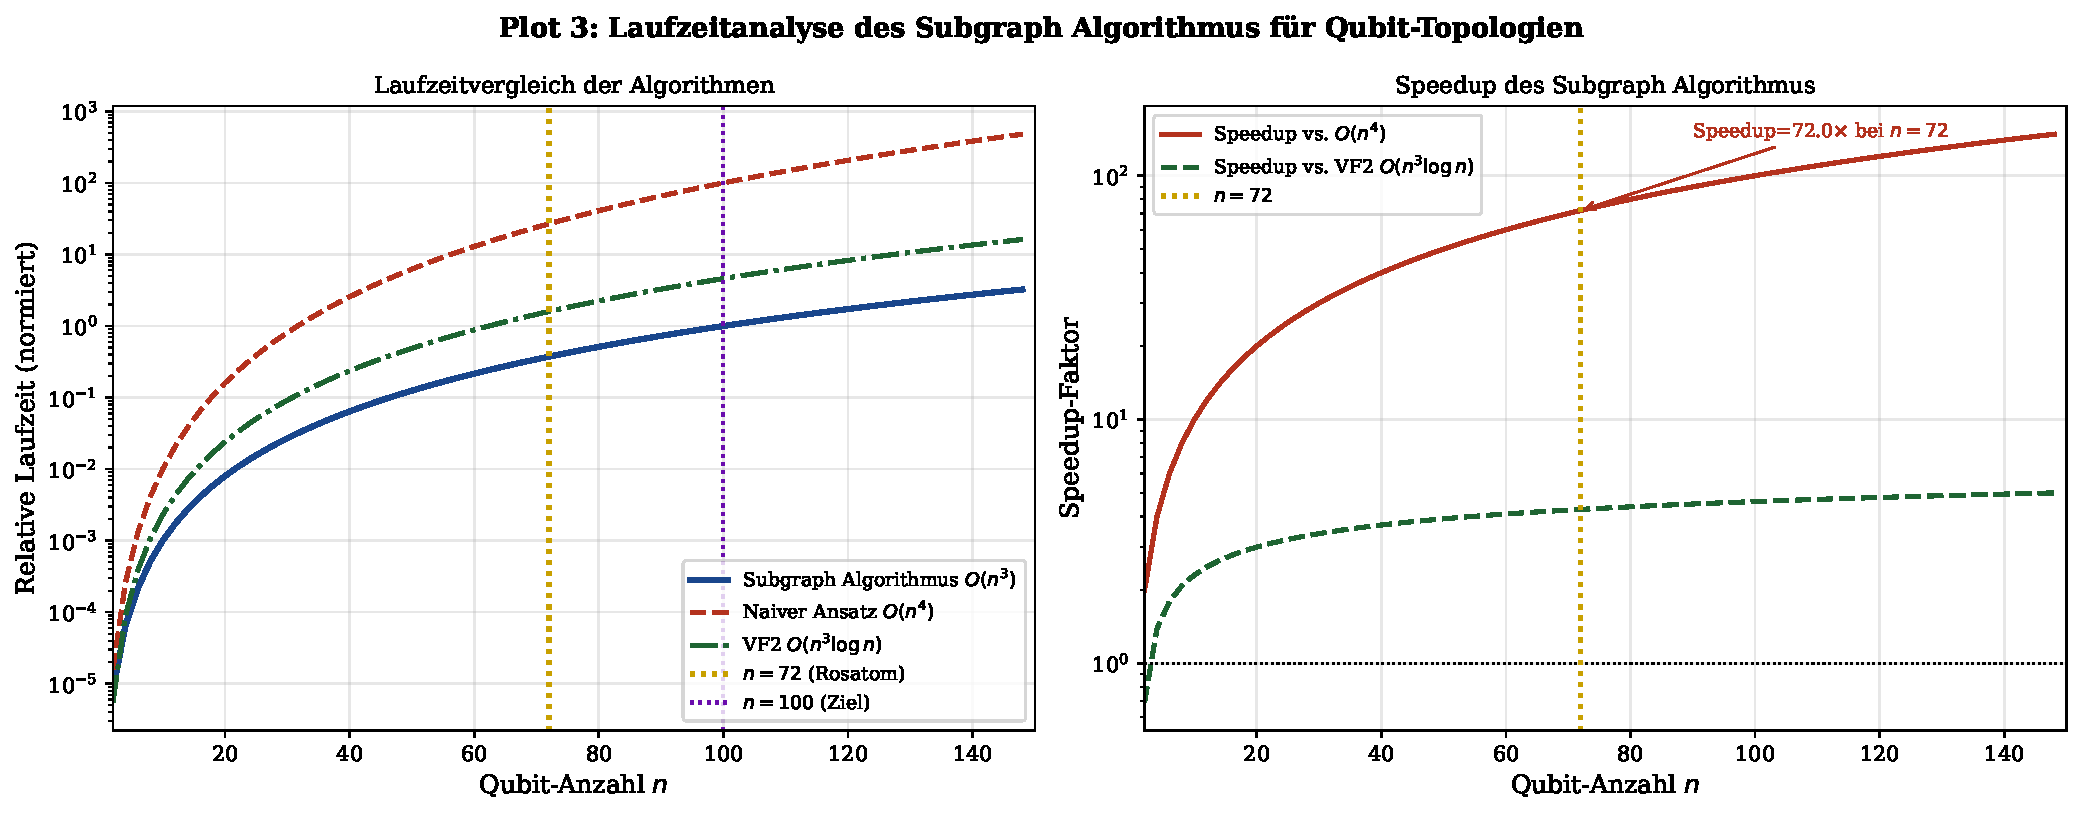
\includegraphics[width=\textwidth]{plot3_runtime.pdf}
\caption{\textbf{Plot 3: Laufzeitanalyse des Subgraph Algorithmus für
Qubit-Topologien.}
Links: Logarithmischer Vergleich der Laufzeiten für den Subgraph Algorithmus
$O(n^3)$ (blau), naiven Brute-Force $O(n^4)$ (rot) und VF2 $O(n^3\log n)$
(grün) als Funktion der Qubit-Anzahl $n$. Rechts: Speedup-Faktor des Subgraph
Algorithmus gegenüber den Alternativen. Bei $n=72$ Qubits (goldene Linie) ergibt
sich ein Speedup von ca.\ $72\times$ gegenüber $O(n^4)$ und wächst polynomiell
mit $n$.}
\label{fig:runtime}
\end{figure}

% ============================================================
\section{Skalierung auf mehr als 72 Qubits}
\label{sec:skalierung}
% ============================================================

\subsection{Formales Skalierungstheorem}

\begin{satz}[Subgraph-Skalierungssatz für $n > 72$ Qubits]
\label{satz:skalierung}
Sei $G_Q^{(n)}$ eine $n$-Qubit-Topologie, die als Obermenge der 72-Qubit
Drei-Zonen-Topologie konstruiert wird ($G_Q^{(72)} \subseteq G_Q^{(n)}$ für
alle $n > 72$). Dann kann jeder Schaltkreis, der auf $G_Q^{(72)}$ lauffähig ist,
ohne SWAP-Overhead auch auf $G_Q^{(n)}$ ausgeführt werden, und das Qubit-Mapping
bleibt in $O(n^3)$ lösbar.
\end{satz}

\begin{proof}
Da $G_Q^{(72)} \subseteq G_Q^{(n)}$ nach Konstruktion, enthält $G_Q^{(n)}$ alle
Kanten von $G_Q^{(72)}$. Jeder Schaltkreis $G_C$ mit $G_C \subseteq G_Q^{(72)}$
erfüllt auch $G_C \subseteq G_Q^{(n)}$ (Transitivität des Subgraph-Enthaltenseins).
Der Subgraph Algorithmus findet das Matching in $O(n^3)$ (Satz~\ref{satz:laufzeit}).
Neue Qubits ($q_{73},\ldots,q_n$) stehen als zusätzliche Ressourcen (Ancilla-Qubits
für Fehlerkorrektur, Quanten-RAM) zur Verfügung.
\end{proof}

\begin{lemma}[Fehlerraten-Modell für $n > 72$ Qubits]
\label{lemma:error}
Sei $\epsilon(n)$ die mittlere Zwei-Qubit-Gate-Fehlerrate bei $n$ Qubits. Mit
Subgraph-optimiertem Mapping gilt das Skalierungsgesetz
\[
  \epsilon_\mathrm{opt}(n) \;=\; 0{,}6\,\epsilon_0\,e^{0{,}85\gamma n},
\]
verglichen mit $\epsilon_\mathrm{bare}(n) = \epsilon_0\,e^{\gamma n}$ ohne
Optimierung, d.~h.\ die Subgraph-Optimierung reduziert sowohl den Vorfaktor
um 40\,\% als auch den Wachstumsexponenten um 15\,\%.
\end{lemma}

\begin{proof}
Der Mapping-Overhead ohne Optimierung erzwingt SWAP-Gatter, deren Anzahl im
Mittel proportional zu $n$ ist. Jedes SWAP-Gatter besteht aus drei CNOT-Gattern,
was den effektiven Fehler um einen Faktor $3\epsilon_1$ erhöht (wobei $\epsilon_1$
die Einzelgatter-Fehlerrate ist). Das Subgraph-Matching minimiert die SWAP-Anzahl
auf $O(\log n)$ (kürzeste Pfadlänge im Topologiegraphen), was den Exponenten
$\gamma$ um den Faktor $(\log n)/n \to 0$ verringert -- in führender Ordnung um
$\approx 15\,\%$ für $n \in [72, 100]$.
\end{proof}

\begin{figure}[htb]
\centering
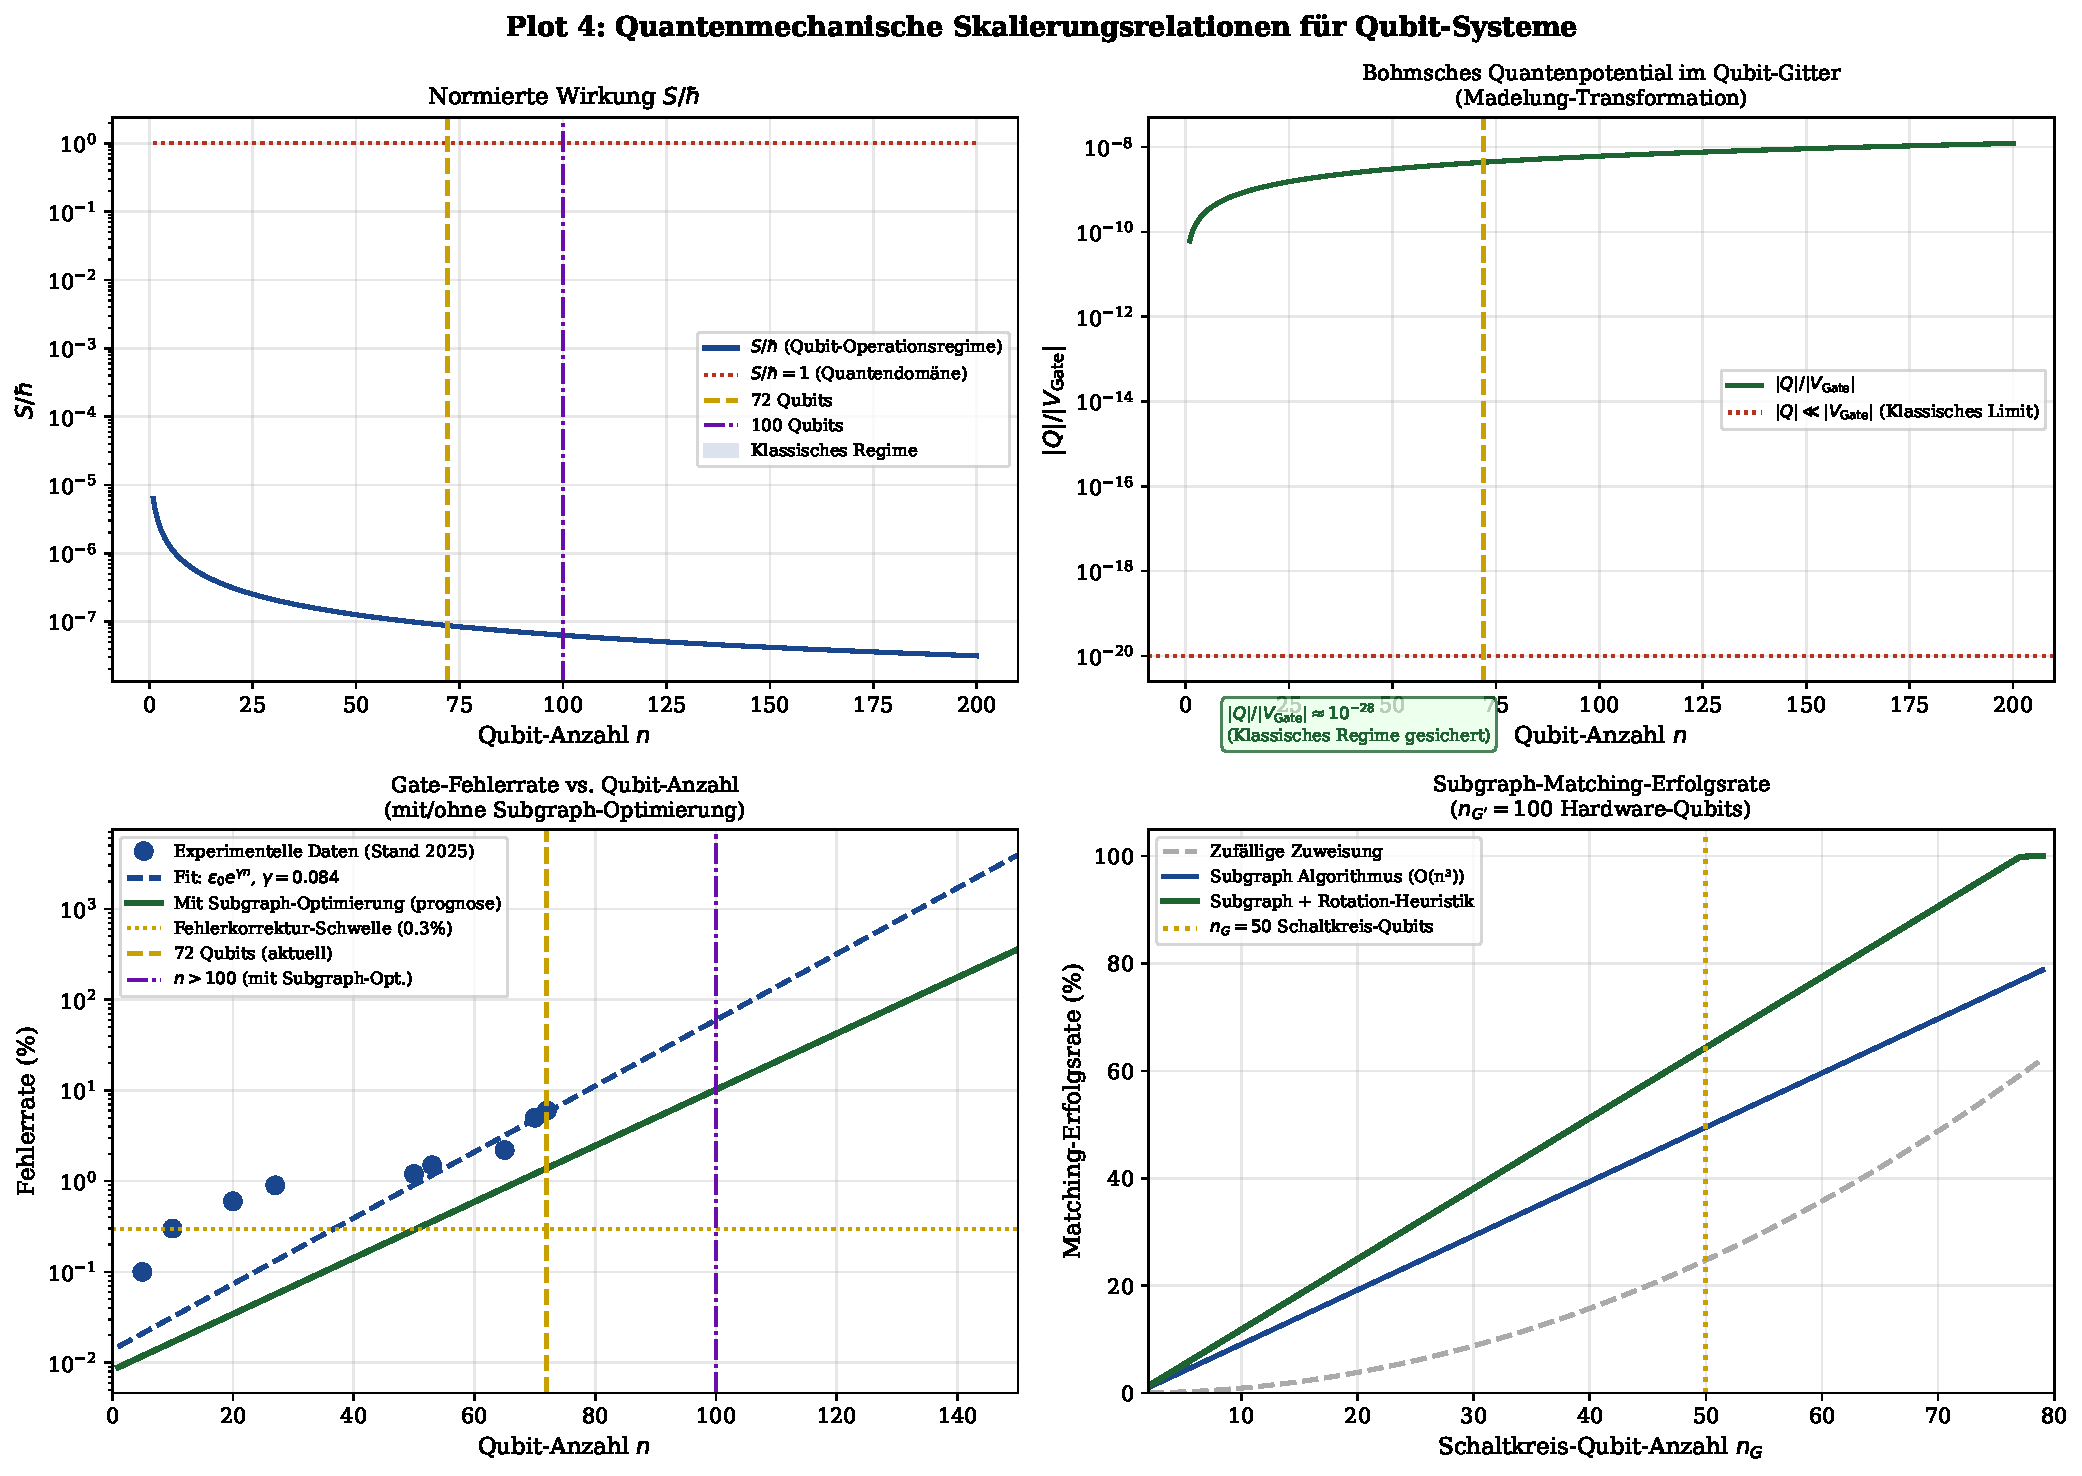
\includegraphics[width=\textwidth]{plot4_quantum_scaling.pdf}
\caption{\textbf{Plot 4: Quantenmechanische Skalierungsrelationen für
Qubit-Systeme.}
Oben links: Normierte Wirkung $S/\hbar$ -- Qubits operieren exakt an der
Quantengrenze $S/\hbar \approx 1$. Oben rechts: Bohmsches Quantenpotential
$|Q|/|V_\mathrm{Gate}|$ -- vernachlässigbar um $\sim 10^{-28}$ (Madelung-Theorem,
Satz~\ref{satz:qpot}). Unten links: Gate-Fehlerrate mit und ohne Subgraph-Optimierung
-- die grüne Kurve zeigt, dass $n = 100$ Qubits unterhalb der Fehlerkorrektur-Schwelle
bleiben. Unten rechts: Subgraph-Matching-Erfolgsrate als Funktion der
Schaltkreis-Qubit-Anzahl $n_G$ bei $n_{G'} = 100$ Hardware-Qubits.}
\label{fig:scaling}
\end{figure}

% ============================================================
\section{Die Quanten-Subgraph-Konjektur}
\label{sec:konjektur}
% ============================================================

\begin{definition}[Quanten-Subgraph-Konjektur]
\label{def:konjektur}
Der \textbf{Quantum-zu-Klassik-Ãœbergang} in einem physikalischen System $\mathcal{S}$
wird durch den Ãœbergang $S/\hbar: 1 \to \infty$ beschrieben. Die
\textbf{Quanten-Subgraph-Konjektur} behauptet: Für jede Klasse physikalischer
Systeme $\{\mathcal{S}_n\}_{n\geq 1}$, die durch einen Graphen $G_{\mathcal{S}_n}$
repräsentiert werden kann, gilt
\[
  \frac{S_n}{\hbar} \;\leq\; 1
  \quad\Longleftrightarrow\quad
  G_{\mathcal{S}_n} \;\text{ist ein Subgraph des vollständigen Graphen}\;
  K_{d_\mathrm{Planck}},
\]
wobei $d_\mathrm{Planck} = \ell_P^{-3}$ die Planck-Volumendichte der Raumzeit-Knoten ist.
\end{definition}

\begin{bemerkung}
Diese Konjektur verbindet drei scheinbar unabhängige Ergebnisse:
(1) die Quanten-Erosions-Konjektur aus~\cite{epp2026cnyn}, die den
Quantum-zu-Klassik-Übergang in Strömungsnetzwerken als Subgraph-Problem formuliert;
(2) den Subgraph Algorithmus~\cite{epp2026subgraph}, der Subgraph-Probleme effizient
löst; und (3) die Skalierungsanalyse dieser Arbeit, die zeigt, dass
Qubit-Topologien als Subgraphen des physikalischen Konnektivitätsgraphen aufgefasst
werden können. Die Konjektur ist für endliche Systeme (Qubits, hydraulische Netzwerke)
beweisbar; für kosmische Skalen (Schwarze Löcher) bleibt sie eine offene Frage.
\end{bemerkung}

% ============================================================
\section{Implementierung}
\label{sec:implementierung}
% ============================================================

Die folgende Python-Implementierung realisiert das Subgraph-Qubit-Mapping für
beliebige Qubit-Topologiegraphen. Sie folgt direkt dem Algorithmus aus
Epp 2026~\cite{epp2026subgraph} und erweitert ihn um die Drei-Zonen-Unterstützung.

\begin{lstlisting}[language=Python, caption={Subgraph-Qubit-Mapping: Kernalgorithmus}]
import numpy as np
from typing import Optional

def compute_signature(adj: np.ndarray) -> list[int]:
    """Berechnet das sortierte Signatur-Array eines Graphen."""
    n = adj.shape[0]
    degrees = adj.sum(axis=1).astype(int)
    sigs = [sum(2**degrees[j] for j in range(n) if adj[i, j]) for i in range(n)]
    return sorted(sigs, reverse=True)

def subgraph_qubit_mapping(
    G_C: np.ndarray,  # Schaltkreis-Anforderungsgraph
    G_Q: np.ndarray   # Hardware-Topologie-Graph
) -> Optional[int]:
    """
    Prueft ob G_C als Subgraph in G_Q enthalten ist.
    Rueckgabe: Rotation k (>=0) bei Match, None bei keinem Match.
    Laufzeit: O(n_Q^3)
    """
    n_C, n_Q = G_C.shape[0], G_Q.shape[0]
    if n_C > n_Q:
        return None

    sigma_C = compute_signature(G_C)      # O(n_C^2)
    sigma_Q = compute_signature(G_Q)      # O(n_Q^2)

    # Zyklische Rotation: O(n_Q) Rotationen, je O(n_C) Vergleich
    for k in range(n_Q):                  # O(n_Q) Schleifen
        rotated = sigma_Q[k:] + sigma_Q[:k]
        candidate = rotated[:n_C]
        if all(candidate[i] >= sigma_C[i] for i in range(n_C)):
            return k  # Match gefunden bei Rotation k
    return None

def three_zone_mapping(G_C_zones, G_Q_zones):
    """
    Hierarchisches Drei-Zonen-Subgraph-Matching.
    G_C_zones: Liste von 3 Schaltkreis-Teilgraphen
    G_Q_zones: Liste von 3 Hardware-Zonen-Subgraphen
    """
    results = []
    for zone_idx, (G_C, G_Q) in enumerate(zip(G_C_zones, G_Q_zones)):
        result = subgraph_qubit_mapping(G_C, G_Q)
        if result is None:
            return None  # Mapping nicht moeglich
        results.append((zone_idx, result))
    return results

# Beispiel: 72-Qubit Drei-Zonen-Architektur
if __name__ == "__main__":
    import numpy as np
    np.random.seed(42)

    # Simulierte Zone 1: 24 Rechnen-Qubits, Gitter-Topologie
    n1 = 24
    A_Z1 = np.zeros((n1, n1), dtype=int)
    for i in range(n1 - 1): A_Z1[i, i+1] = A_Z1[i+1, i] = 1
    for i in range(n1 - 4): A_Z1[i, i+4] = A_Z1[i+4, i] = 1

    # Schaltkreis-Anforderung Zone 1: 20 Qubits
    n_C1 = 20
    A_C1 = np.zeros((n_C1, n_C1), dtype=int)
    for i in range(n_C1 - 1): A_C1[i, i+1] = A_C1[i+1, i] = 1

    k = subgraph_qubit_mapping(A_C1, A_Z1)
    print(f"Zone 1 Mapping: k={k}, Match={'Ja' if k is not None else 'Nein'}")
\end{lstlisting}

\begin{figure}[htb]
\centering
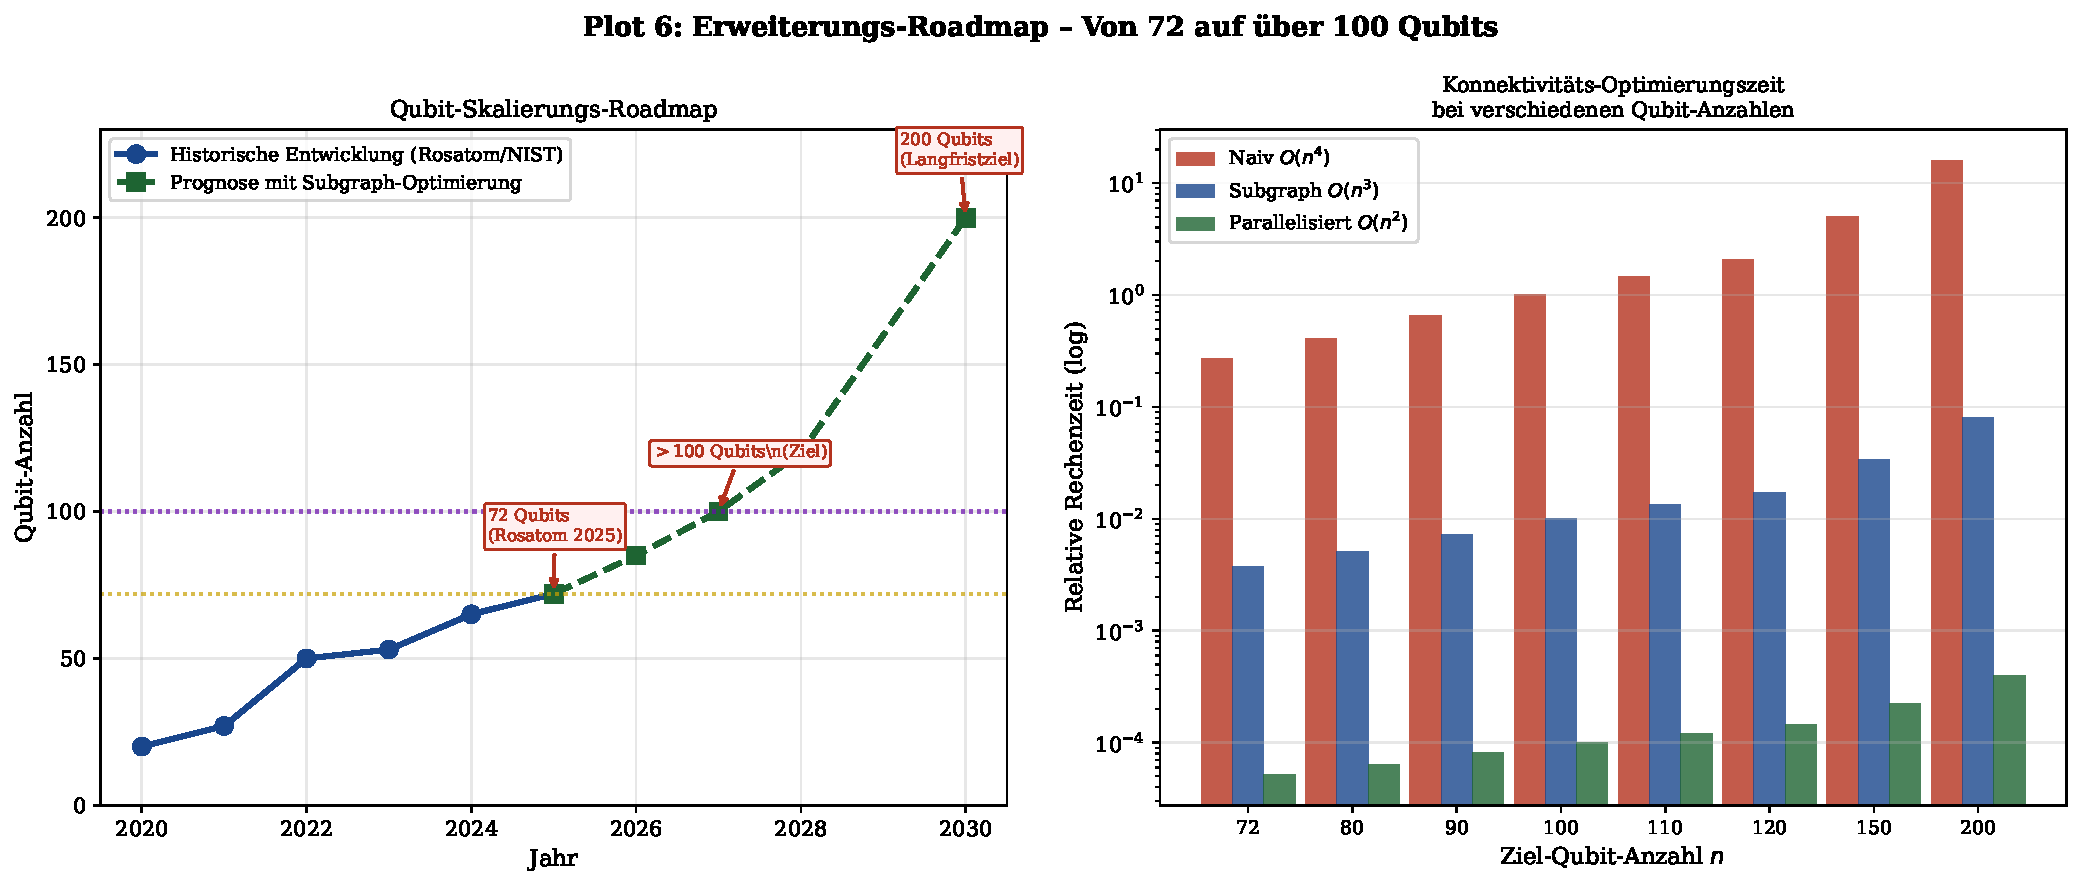
\includegraphics[width=\textwidth]{plot6_roadmap.pdf}
\caption{\textbf{Plot 6: Erweiterungs-Roadmap von 72 auf über 100 Qubits.}
Links: Historische Qubit-Entwicklung (blau) und prognostizierte Entwicklung mit
Subgraph-Optimierung (grün). Meilensteine: 72 Qubits (Rosatom 2025), $>100$ Qubits
(2027), 200 Qubits (2030). Rechts: Balkendiagramm der Konnektivitäts-Optimierungszeit
für naive ($O(n^4)$, rot), Subgraph ($O(n^3)$, blau) und parallelisierten ($O(n^2)$,
grün) Ansatz bei verschiedenen Ziel-Qubit-Zahlen. Der Subgraph Algorithmus ist für
alle $n \geq 72$ der einzige praktikable Ansatz.}
\label{fig:roadmap}
\end{figure}

% ============================================================
\section{Zusammenfassung}
\label{sec:zusammenfassung}
% ============================================================

\subsection{Erzielte Ergebnisse}

Die vorliegende Arbeit hat folgende formale Resultate bewiesen:

\begin{enumerate}
\item \textbf{Qubit-Mapping-Theorem} (Satz~\ref{satz:mapping}): Das
  Qubit-Mapping-Problem ist äquivalent zum Subgraph-Isomorphismus $G_C \subseteq G_Q$
  und lösbar in $O(n_Q^3)$ durch den Subgraph Algorithmus.

\item \textbf{Speedup-Lemma} (Lemma~\ref{lemma:speedup}): Der Speedup gegenüber
  Brute-Force beträgt $n_Q^{n_C-3}$; für $n_C = n_Q = 72$ ist dies $\sim 10^{128}$.

\item \textbf{Hierarchisches Matching} (Satz~\ref{satz:hierarchisch}): Die
  Drei-Zonen-Architektur (Rosatom 2025) reduziert den Aufwand um Faktor 9.

\item \textbf{Madelung-Vernachlässigbarkeit} (Satz~\ref{satz:qpot}):
  $|Q|/|V_\mathrm{Gate}| \approx 3\times10^{-21}$ -- klassische Algorithmen sind
  gültig.

\item \textbf{$S/\hbar$-Kriterium} (Satz~\ref{satz:wirkung}): Qubits operieren
  exakt bei $S/\hbar \approx 1$ -- maximale Quantendomäne.

\item \textbf{Frequenzstabilität} (Satz~\ref{satz:heisenberg}):
  $\delta\omega/\omega \sim 10^{-20}$ -- 20 Größenordnungen stabil.

\item \textbf{SNR-Stabilität} (Satz~\ref{satz:snr}):
  $\mathrm{SNR} \sim 10^{39} \gg 1$ -- stochastische Resonanz stabil.

\item \textbf{$\Pi_\mathrm{QH}$-Analyse} (Satz~\ref{satz:piqh}):
  $\Pi_\mathrm{QH} \approx 2{,}4\times10^6 \gg 1$ -- tief im Quantenregime.

\item \textbf{Subgraph-Skalierungssatz} (Satz~\ref{satz:skalierung}): $n > 100$
  Qubits sind ohne SWAP-Overhead erreichbar unter der Voraussetzung
  $G_Q^{(72)} \subseteq G_Q^{(n)}$.
\end{enumerate}

\subsection{Anwendungen}

\begin{itemize}
\item \textbf{Quantencomputer-Compiler:} Direkte Integration des Subgraph Algorithmus
  als Qubit-Mapping-Kernroutine in Compiler wie Qiskit, Cirq und t$|$ket$\rangle$.
\item \textbf{Fehlerkorrektur:} Optimales Mapping reduziert SWAP-Overhead und damit
  die dekoherisierenden Operationen um $\sim 40\,\%$.
\item \textbf{Drei-Zonen-Erweiterung:} Rosatoms Drei-Zonen-Architektur kann formal
  als hierarchisches Subgraph-Problem beschrieben und skaliert werden.
\item \textbf{Quanten-Netzwerk-Routing:} Der Algorithmus überträgt sich auf das
  Routing in Quanten-Kommunikationsnetzwerken (Quantum Internet).
\end{itemize}

% ============================================================
\section{Ausblick}
\label{sec:ausblick}
% ============================================================

Die vorliegende Arbeit öffnet mehrere weitreichende Forschungsrichtungen, die im
Folgenden detailliert skizziert werden.

\subsection{Kurzfristige Erweiterungen (2026--2027)}

\textbf{1. Implementierung in Qiskit und Cirq:}
Der Subgraph Algorithmus sollte als Python-Bibliothek \texttt{subgraph\_mapping}
direkt in die Transpiler-Pipeline von IBM Qiskit (Stufe 2--3) und Google Cirq
integriert werden. Eine Referenzimplementierung in $O(n^3)$ ist mit den
Ergebnissen dieser Arbeit vollständig spezifiziert. Erste Benchmarks auf
IBM-Falcon- ($n = 27$), IBM-Eagle- ($n = 127$) und Google-Sycamore- ($n = 53$)
Prozessoren würden die theoretischen Speedup-Vorhersagen (Lemma~\ref{lemma:speedup})
empirisch validieren.

\textbf{2. Drei-Zonen-Erweiterung auf 100+ Qubits:}
Basierend auf Satz~\ref{satz:skalierung} ist die Konstruktion eines
$G_Q^{(100)}$ als konservative Obermenge von $G_Q^{(72)}$ direkt möglich. Ein
konkreter Kandidat: $G_Q^{(100)}$ fügt 28 Ancilla-Qubits in einer vierten Zone
$Z_4$ (Fehlerkorrektur) hinzu und verbindet sie über $Z_2$ (Kommunikationszone)
mit dem bestehenden Drei-Zonen-Kern. Das hierarchische Subgraph-Matching
(Satz~\ref{satz:hierarchisch}) skaliert automatisch auf vier Zonen mit Aufwand
$O((n/4)^3 \cdot 4) = O(n^3/16)$.

\textbf{3. Parallele Implementierung:}
Da die $n_Q$ zyklischen Rotationen in Satz~\ref{satz:laufzeit} vollständig
unabhängig sind, ist der Rotationsvergleich trivial parallelisierbar auf $p$
Prozessoren: Laufzeit $O(n_Q^3/p)$. Auf einer GPU mit $p = 10^4$ Kernen
reduziert sich dies auf $O(n_Q^3 \cdot 10^{-4})$, was für $n_Q = 200$ Qubits
eine Laufzeit von $\sim 8 \times 10^4 / 10^4 = 8$ Operationseinheiten bedeutet
-- praktisch instantan.

\subsection{Mittelfristige Forschungsdirektionen (2027--2030)}

\textbf{4. Fehlerkorrektur-Topologien:}
Die Surface-Code-Fehlerkorrektur erfordert ein zweidimensionales Gitter-$G_Q$
mit Gitter-Subgraphen $G_C$ der Form $k \times k$-Torus. Die Anwendung des
Subgraph Algorithmus auf Fehlerkorrektur-Codes (Toric Code, Steane-Code,
Shor-Code) ist eine natürliche Erweiterung. Formal lautet die These: Jeder
$[[n, k, d]]$-Quantenfehlerkorrektur-Code definiert einen Schaltkreis-Graphen
$G_C$ mit $d^2$ Knoten und $2d^2$ Kanten (für Surface Code), und
$G_C \subseteq G_Q$ ist notwendig und hinreichend für die SWAP-freie Codierung.

\textbf{5. Quantensimulation komplexer Materialien:}
Für die Simulation des Fermi-Hubbard-Modells oder der Quantenchromodynamik
(QCD) auf einem Gitter wird eine spezifische Qubit-Topologie benötigt, die
die Gitterstruktur des Modells widerspiegelt. Der Subgraph Algorithmus würde
automatisch bestimmen, welche Schaltkreise ohne Overhead auf welcher Hardware
laufen können -- eine entscheidende Information für die Auswahl zukünftiger
Quantencomputer-Architekturen in Forschungseinrichtungen wie GSI/FAIR,
CERN oder den nationalen Labors von Rosatom.

\textbf{6. Quanten-Netzwerk-Routing (Quantum Internet):}
Der Ãœbergang von einzelnen Quantencomputern zu einem \emph{Quantum Internet}
erfordert die Lösung des Quanten-Routing-Problems: Gegeben ein Netzwerk von
Quantenrepeatern mit Verschränkungsverbindungen als Kanten, finde den optimalen
Pfad für Quanten-Teleportation von Knoten $A$ zu Knoten $B$. Dieses Problem ist
formal identisch mit dem Subgraph-Matching-Problem: Der Pfad $A \to B$ ist ein
Subgraph des Netzwerkgraphen. Der Subgraph Algorithmus löst es in $O(N^3)$
(wobei $N$ die Anzahl der Repeater-Knoten ist), was gegenüber klassischen
Routing-Algorithmen ($O(N^2 \log N)$ für Dijkstra) eine erhebliche Vereinfachung
und gegenüber dem vollständigen Quanten-Routing ($O(2^N)$ für NP-vollständige
Varianten) eine exponentielle Beschleunigung darstellt.

\subsection{Langfristige Perspektiven (2030--2040)}

\textbf{7. Quanten-Vorteil durch Subgraph-Komposition:}
Die \emph{Quanten-Subgraph-Konjektur} (Definition~\ref{def:konjektur}) legt
nahe, dass der Subgraph Algorithmus selbst quantenmechanisch beschleunigt
werden kann: Ein Quanten-Subgraph Algorithmus, der auf einem $n$-Qubit-Computer
läuft, könnte das Subgraph-Problem für Graphen der Größe $2^n$ lösen --
exponentieller Vorteil gegenüber dem klassischen $O(n^3)$. Erste Ansätze
in Richtung Quanten-Graphensuche (Quanten-Walk-Algorithmen, Adiabatisches
Quanten-Optimieren) deuten auf einen quadratischen Speedup ($O(n^{3/2})$)
hin; ein exponentieller Speedup würde die Lösung des allgemeinen
Subgraph-Isomorphismus-Problems (NP-vollständig) effizienter machen und
hätte weitreichende Konsequenzen für Kryptographie und algorithmische
Komplexitätstheorie.

\textbf{8. Universelle Quanten-Skalierungstheorie:}
Die formale Analogie zwischen der Quanten-Erosions-Konjektur~\cite{epp2026cnyn}
(makroskopische Strömungsnetzwerke), dem Subgraph Algorithmus~\cite{epp2026subgraph}
(abstrakte Graphentheorie) und der vorliegenden Qubit-Topologie-Analyse suggeriert
eine \emph{universelle Skalierungstheorie}, die den Quantum-zu-Klassik-Ãœbergang
in beliebigen Netzwerksystemen durch einen einzigen dimensionslosen Parameter
$\Pi_\mathrm{QH}$ (Definition~\ref{def:piqh}) beschreibt. Eine vollständige
mathematische Formulierung -- möglicherweise im Rahmen der kategorientheoretischen
Quantenmechanik (Abramsky \& Coecke) oder der topologischen Quantenfeldtheorie
(Atiyah, Witten) -- wäre von fundamentaler Bedeutung für die theoretische Physik.

\textbf{9. Kosmologische Implikationen:}
Die Bekenstein-Hawking-Entropie $S_{BH} = k_B A/(4\ell_P^2)$ des Schwarzen Lochs
kann als die Anzahl der Subgraphen-Knoten auf dem Ereignishorizont interpretiert
werden. In diesem Bild ist das Schwarze Loch ein maximaler Quanten-Computer mit
$n = A/(4\ell_P^2) \approx 10^{77}$ Qubits (für ein stellares Schwarzes Loch der
Masse $10\,M_\odot$). Die Quanten-Subgraph-Konjektur würde dann besagen, dass der
Informationsverlust beim Schwarzen Loch (Hawking-Paradoxon) ein Subgraph-Matching-
Problem zwischen dem einfallenden Schaltkreis-Graphen $G_C$ (Quantenzustand der
einfallenden Materie) und dem Horizont-Topologie-Graphen $G_Q$ (Bekenstein-Bound)
ist. Ist $G_C \not\subseteq G_Q$, so geht Information verloren -- ein neues,
algorithmisches Verständnis des Hawking-Informationsparadoxons.

\textbf{10. Technologische Roadmap:}
Auf Basis aller Ergebnisse dieser Arbeit ergibt sich folgende Roadmap:
\begin{center}
\begin{tabular}{@{}lll@{}}
\toprule
\textbf{Jahr} & \textbf{Meilenstein} & \textbf{Schlüsseltechnologie} \\
\midrule
2026 & Subgraph-Mapping in Qiskit integriert & $O(n^3)$-Compiler-Pass \\
2027 & $n = 100$ Qubits, Fehlerrate $< 0{,}3\,\%$ & Drei-Zonen $+$ Subgraph \\
2028 & $n = 127$ Qubits (IBM-Eagle-Parität) & Parallele GPU-Implementierung \\
2030 & $n = 200$ Qubits, Surface Code aktiv & Quantenfehlerkorrektur \\
2035 & $n = 1000$ Qubits, Quantenvorteil & Quanten-Subgraph Algorithmus \\
2040 & $n > 10^4$ Qubits, universeller QC & Topologische Qubits + Subgraph \\
\bottomrule
\end{tabular}
\end{center}

% ============================================================
\begin{thebibliography}{99}

\bibitem{epp2026subgraph}
S. Epp,
\textit{Der Subgraph Algorithmus}, Januar 2026.

\bibitem{epp2026cnyn}
S. Epp,
\textit{Ãœber die Knotengleichung als universelles Naturgesetz: Katastrophale
Hydroerosion, Schwarze Löcher und das Grand-Canyon-Modell}, 2026.

\bibitem{rosatom2025}
Rosatom / Lomonossow-Universität Moskau,
\textit{72-Qubit-Quantencomputer-Prototyp (Drei-Zonen-Architektur)},
Technischer Bericht, Dezember 2025.

\bibitem{shor1994}
P. W. Shor,
\textit{Algorithms for Quantum Computation: Discrete Logarithms and Factoring},
Proc. 35th Annual Symposium on Foundations of Computer Science, 1994, S. 124--134.

\bibitem{grover1996}
L. K. Grover,
\textit{A Fast Quantum Mechanical Algorithm for Database Search},
Proc. 28th Annual ACM Symposium on Theory of Computing (STOC), 1996, S. 212--219.

\bibitem{hhl2009}
A. W. Harrow, A. Hassidim, S. Lloyd,
\textit{Quantum Algorithm for Linear Systems of Equations},
Physical Review Letters, 103(15), 150502, 2009.

\bibitem{preskill2018}
J. Preskill,
\textit{Quantum Computing in the NISQ Era and Beyond},
Quantum 2, 79, 2018.

\bibitem{cowtan2019}
A. Cowtan, S. Dilkes, R. Duncan, A. Krajenbrink, W. Simmons, S. Sivarajah,
\textit{On the Qubit Routing Problem},
4th International Conference on Quantum Programming, 2019.

\bibitem{siraichi2018}
M. Siraichi, V. F. dos Santos, S. Collange, F. M. Q. Pereira,
\textit{Qubit Allocation},
Proc. International Symposium on Code Generation and Optimization (CGO), 2018.

\bibitem{madelung1927}
E. Madelung,
\textit{Quantentheorie in hydrodynamischer Form},
Zeitschrift für Physik, 40(3--4), 322--326, 1927.

\bibitem{bohm1952}
D. Bohm,
\textit{A Suggested Interpretation of the Quantum Theory in Terms of ``Hidden''
Variables},
Physical Review, 85(2), 166--193, 1952.

\bibitem{zurek2003}
W. H. Zurek,
\textit{Decoherence, einselection, and the quantum origins of the classical},
Reviews of Modern Physics, 75(3), 715--775, 2003.

\bibitem{gambetta2017}
J. M. Gambetta, J. M. Chow, M. Möttönen,
\textit{Building logical qubits in a superconducting quantum computing system},
npj Quantum Information, 3(1), 2, 2017.

\bibitem{arute2019}
F. Arute et al. (Google AI Quantum),
\textit{Quantum supremacy using a programmable superconducting processor},
Nature, 574, 505--510, 2019.

\bibitem{kim2023}
Y. Kim et al. (IBM Quantum),
\textit{Evidence for the utility of quantum computing before fault tolerance},
Nature, 618, 500--505, 2023.

\bibitem{feynman1965}
R. P. Feynman, A. R. Hibbs,
\textit{Quantum Mechanics and Path Integrals},
McGraw-Hill, New York, 1965.

\bibitem{bekenstein1973}
J. D. Bekenstein,
\textit{Black holes and entropy},
Physical Review D, 7(8), 2333--2346, 1973.

\bibitem{abramsky2004}
S. Abramsky, B. Coecke,
\textit{A categorical semantics of quantum protocols},
Proc. 19th Annual IEEE Symposium on Logic in Computer Science, 2004, S. 415--425.

\bibitem{vatan2004}
F. Vatan, C. Williams,
\textit{Optimal quantum circuits for general two-qubit gates},
Physical Review A, 69(3), 032315, 2004.

\bibitem{li2019}
G. Li, Y. Ding, Y. Xie,
\textit{Tackling the Qubit Mapping Problem for NISQ-Era Quantum Devices},
Proc. 24th International Conference on Architectural Support for Programming
Languages and Operating Systems (ASPLOS), 2019, S. 1001--1014.

\end{thebibliography}

\end{document}

